\documentclass[]{article}
\usepackage[hidelinks]{hyperref}

\usepackage{listings}
\usepackage{color}
\usepackage{amsmath}
\usepackage{amssymb}
\usepackage{mathtools}
\usepackage[mode=buildnew]{standalone}
\usepackage{tikz}
\usepackage{pgfplots}
\usepackage{caption}
\usepackage{subcaption}
\usepackage{multirow}
\usepackage{amsthm}
\pgfplotsset{compat=newest}


\definecolor{dkgreen}{rgb}{0,0.6,0}
\definecolor{gray}{rgb}{0.5,0.5,0.5}
\definecolor{mauve}{rgb}{0.58,0,0.82}

\lstset{frame=tb,
	language=Java,
	aboveskip=3mm,
	belowskip=3mm,
	showstringspaces=false,
	columns=flexible,
	basicstyle={\small\ttfamily},
	numbers=none,
	numberstyle=\tiny\color{gray},
	keywordstyle=\color{blue},
	commentstyle=\color{dkgreen},
	stringstyle=\color{mauve},
	breaklines=true,
	breakatwhitespace=true,
	tabsize=3
}

\newcommand{\argmax}[1]{\underset{#1}{\operatorname{arg}\,\operatorname{max}}\;}
\newcommand\Tstrut{\rule{0pt}{2.6ex}}         % = `top' strut
\newcommand\Bstrut{\rule[-0.9ex]{0pt}{0pt}}   % = `bottom' strut


%opening
\title{Payment Rules through \\ Discriminant-Based Classifiers}
\author{ by Paul D\"utting, Felix Fischer, Pichayut Jirapinyo, John K. Lai, \\Benjamin Lubin and David C. Parkes \\ \\ Manuscript by Nicolas K\"uchler}
\date{\today}

\begin{document}

\maketitle

\section{Introduction}
\emph{Payment Rules through Discriminant-Based Classifiers} is a paper from 2012 where Paul D\"utting, Felix Fischer, Pichayut Jirapinyo, John K. Lai, Benjamin Lubin and David C. Parkes present a new method for constructing payment rules in \emph{Mechanism Design}.

\noindent In \emph{Mechanism Design} we are looking at situations where agents hold private informations about their preferences over different outcomes. 
Agents submit reports and the mechanism chooses an outcome and a payment.


\subsection{Classical Approach for Mechanism Design}
The classical approach is to start by imposing an incentive compatibility IC constraint (e.g. DSIC: dominant-strategy IC or BNIC: Bayesian-Nash IC) ensuring that agents report their preferences in equilibrium truthfully. Subject to that constraint, an outcome- and a payment rule are chosen. The classical approach however, brings some challenges:


\paragraph{Analytical Complexity} It is difficult to find optimal mechanisms in \emph{multi-dimensional domains}, where agents private information is described through more than a single number.

\paragraph{Exclusion of Mechanisms} Incentive compatibility as a hard constraint might preclude mechanisms with useful economic properties.

\paragraph{Computational Complexity} Payment rules can become computational intractable.


\subsection{New Approach for Mechanism Design}
In the new approach presented in the paper, we start from a given outcome rule $g$ (e.g. optimal outcome rule) and a distribution over agent type profiles $D$. Then we use machine learning ML to identify a payment rule $p$ that has good incentive properties relative to this outcome rule $g$. Instead of insisting on a hard incentive compatibility constraint, we minimize a metric called expected ex-post regret. This measures an agents regret reporting truthfully rather than any other false report that could have led to a personally preferred outcome.

\begin{figure}[h]
	\begin{tabular}{|c|c|}
		\hline
	\begin{subfigure}{0.46\textwidth}
			\begin{tabular}{r l} 
			\multicolumn{2}{l}{\textbf{Classical Approach}} \\
			1.	& Impose IC constraint \\ 
			2.	& Design outcome- and payment  \\ 
				& rule subject to IC constraint
			\end{tabular} 
		\begin{center}
		\includestandalone[width=1.05\textwidth]{res/oldApproach}
	\end{center}
		\label{fig:oldApproach}
	\end{subfigure} &
	\begin{subfigure}{.46\textwidth}
		\begin{tabular}{r l} 
			\multicolumn{2}{l}{\textbf{New Approach}} \Tstrut \\
			1.	& Define outcome rule\\ 
			2.	& Define type distribution  \\ 
			3.	& Use ML to find payment rule \\ 
		\end{tabular} 
		\begin{center}
		\includestandalone[width=0.9\textwidth]{res/newApproach}
		\end{center}
		\label{fig:newApproach}
	\end{subfigure} \\
\hline
\end{tabular}
\caption{Comparison of the two approaches for \emph{Mechanism Design}.}
\label{fig:comparison}
\end{figure}


\subsection{Structure}
After introducing the new approach, the authors show the connection between finding a payment rule in \emph{Mechanism Design} and the \emph{Multi-Class Classification} problem of \emph{Machine Learning}. Later they present a framework using \emph{Structural Support Vector Machines} and apply it in experiments to two different domains. 

\section{Preliminaries}
\subsection{Ex-Post Regret}
The \emph{ex-post regret} an agent has for truthfully reporting in a given instance is the amount by which its utility could be increased through a misreport. Formally, the \emph{ex-post regret} of agent i, given true type $\theta_{i} \in \Theta_{i}$ and the other agents reported types $\theta'_{-i} \in \Theta_{-i}$ is:

\begin{equation*}
rgt_{i}(\theta_{i},\theta'_{-i}) = \max\limits_{\theta'_{i} \in \Theta_{i}} 
\underbrace{u_{i}((\theta'_{i}, \theta'_{-i}), \theta_{i})}_{\mathclap{\text{utility misreport}}}
- \underbrace{u_{i}((\theta_{i}, \theta'_{-i}), \theta_{i})}_{\mathclap{\text{utility truthful report}}}
\end{equation*}

\noindent When a mechanism has zero \emph{ex-post regret} for all inputs $(\theta_{i}, \theta_{-i})$, then it is \emph{strategyproof}. Apart from that, \emph{ex-post regret} does not have any further known direct implications for equilibrium properties. The support for \emph{expected ex-post regret} rather comes from a simple model, where agents face a certain cost for strategic behaviour. If this cost is higher than the expected gain, then the agents are assumed to behave truthfully.


\section{Payment Rules from Multi-Class Classifiers}

To show how finding a payment rule with good incentive properties is connected with the multi-class classification problem is really the essence of the paper but also not that straightforward to understand. Before building the connection, we start by looking at characteristics of a strategyproof mechanism and introduce the concept of a multi-class classifier.

\subsection{Truthful Mechanisms}
It is known that a mechanism is truthful if and only if two properties hold:

\paragraph{Agent-Independent Price}
Payment $p_{i}$ is independent of agent $i$'s reported type $\theta_{i}$:
\begin{equation*}
p_{i}(\theta) = t_{i}(\theta_{-i}, g_{i}(\theta)) \quad \quad \forall i \in N
\end{equation*}


\paragraph{Agent-Optimizing Outcome} 
The chosen outcome $g_{i}(\theta)$ simultaneously maximizes the utility of all agents:
\begin{equation*}
g_{i}(\theta) \in \argmax{o_{i} \in \Omega_{i}} v_{i}(\theta_{i}, o_{i}) - t_{i}(\theta_{-i}, o_{i}) \quad \quad \forall i \in N
\end{equation*}

\subsection{Multi-Class Classifiers}

A multi-class classifier takes an input $x$ and finds the best fitting class $y$:

\begin{equation*}
h_{w}(x) \in \argmax{y \in Y} f_{w}(x,y)
\end{equation*}

\noindent in our case the classifier is parametrized by a learned weight vector $w \in \mathbb{R}^{m}$.
Learning the classifier $h_{w}$ is nothing more than learning the function $f_{w}$.

\paragraph{Classifier in Mechanism Design} It might sound really surprising that even though we are eventually looking for a payment rule $p$, we try to find a classifier for the outcome $o_{i} = g_{i}(\theta)$. So in our case the classifier receives as input a type profile  $\theta$ and classifies an outcome $o_{i}$:

\begin{equation*}
h_{w}(\theta) \in \argmax{o_{i} \in \Omega_{i}} f_{w}(\theta,o_{i})
\end{equation*}

\subsection{Connection}
Assuming agent symmetry, we build the connection by focusing on a partial outcome rule $g_{1}$ and a classifier $h_{w}$ for agent 1. Agent symmetry means informally that without loss of generality the problem is the same for every agent and it is thus enough to only consider it from the perspective of one agent.

\noindent Now let's look at the connection between truthful mechanisms and multi-class classifiers. 


\noindent Comparing classifier and \emph{agent-optimizing outcome} property we see that they are really similar;
both are looking for an optimal outcome $o_{i}$ in a function of a type profile $\theta$.

\noindent These similarities become even more striking when we consider only classifiers with a special discriminant-based structure of value - price, resembling utility of an agent:

\small
\begin{equation*}
\begin{aligned}
& \text{\emph{Agent-Optimizing Property:}} & g_{1}(\theta) \in \argmax{o_{1} \in \Omega_{1}} & & v_{1}(\theta_{1}, o_{1}) & & - && t_{1}(\theta_{-1}, o_{1})\\
& \text{\emph{Discriminant-Based Classifier:}} & h_{w}(\theta) \in \argmax{o_{1} \in \Omega_{1}} &  & w_{1}v_{1}(\theta_{1}, o_{1})& & + && w_{-1}^{T}\psi(\theta_{-1}, o_{1})  \\
\end{aligned}
\end{equation*}
\normalsize

\noindent Feature mapping function $\psi$ maps $\theta_{-1}$ and $o_{1}$ into a single vector $\in \mathbb{R}^{m}$.


\noindent Due to this discriminant-based structure, learning the function $f_{w}$, becomes learning the payment rule $p_{w}$. We can see this by defining the associated price function:


\begin{equation*}
 t_{w}(\theta_{-1}, o_{1}) = - \frac{1}{w_{1}} w_{-1}^T \psi(\theta_{-1},o_{1})
\end{equation*}

\noindent And now with agent symmetry, we can obtain the complete payment rule $p_{w}(\theta)$ by plugging in this price function from each agent:

\begin{equation*}
p_{w}(\theta) = (t_{w}(\theta_{-1},g_{1}(\theta)), t_{w}(\theta_{-2},g_{2}(\theta)),..., t_{w}(\theta_{-n},g_{n}(\theta)))
\end{equation*}

\noindent The \emph{agent-independent price} property of a truthful mechanism can be directly inferred from the associated price function $t_{w}(\theta_{-1}, o_{1})$, because it doesn't depend on an agents own report $\theta_{1}$.

\newpage
\subsection{Truthful Mechanisms with a Perfect Classifier}
To complete the connection between strategyproof mechanisms and multi-class classifiers we take a brief look at a Theorem from the paper:

\paragraph{Theorem 3.2}  Let $g$ be an agent symmetric outcome rule, $h_{w}$ an admissible classifier, and $p_{w}$ the payment rule corresponding to $h_{w}$. If $h_{w}$ is a perfect classifier for the partial outcome rule $g_{1}$, then the mechanism $(g,p_{w})$ is strategyproof.

\begin{center}
	$h_{w}$ is a \emph{perfect classifier} for $g_{1}$ $\Rightarrow$ mechanism $(g,p_{w})$ is strategyproof
\end{center}

\noindent A classifier is called a \emph{perfect classifier} if it is able to classify all inputs correctly. In terms of our problem that means the trained classifier always selects the same outcome as the outcome rule.

\noindent Unfortunately identified mechanisms $(g,p_{w})$ are hardly ever strategyproof because a perfect classifier is rather rare. 
However, the authors show that the result extends gracefully to situations where no perfect classifier is found by relating \emph{expected ex-post regret} of a mechanism to a measure of the generalization error of a classifier for $g$. Essentially this allows us to see, that minimizing the generalization error of the classifier (minimizing the number of miss-classifications), leads to minimizing the \emph{expected ex-post regret} of the mechanism.


\subsection{Example Single Item Auction}
To gain some more intuition, let's consider a simple mechanism; the \emph{Single Item Auction}. There are two possible outcomes  $o_{i}\in\{0,1\}$ for each bidder, either the item is allocated to agent $i$ or it is not. Each agent reports his type  $\theta_{i}$, representing his value for the item, to the mechanism and the outcome rule allocates the item to the agent with the highest value.


\noindent The structure of the classifier $h_{w}(\theta) \in \argmax{o_{1} \in \Omega_{1}} w_{1}v_{1}(\theta_{1}, o_{1})+ w_{-1}^{T}\psi(\theta_{-1}, o_{1})$ has to make sure that the outcome $o_{i}$ matching the outcome rule $g(\theta)$ has to be optimal for every agent $i$. Concretely this means when agent 1 has a higher valuation for the item than the other agents, then the outcome $o_{1} = 1$ (allocate the item to agent 1) needs to maximize the classifier. Otherwise outcome $o_{1}=0$ (not allocate the item to agent 1) needs to maximize the classifier.

\noindent In our example this can be achieved by setting: 
\begin{equation*}
w_{1} = 1 \text{\quad and\quad} w_{-1}^T \psi(\theta_{-1},o_{1})= 
\begin{cases}
- max(\theta_{-1})& \text{if } o_{1} = 1\\
0              & \text{if } o_{1} = 0
\end{cases}
\end{equation*}

\noindent As we can see when plugging this into the associated price function  $t_{w}(\theta_{-1}, o_{1}) = - \frac{1}{w_{1}} w_{-1}^T \psi(\theta_{-1},o_{1})$, this leads to the well known second price payment rule.

\newpage
\noindent To clarify lets consider a small \emph{Single Item Auction} instance with two agents. The optimal outcome is $o_{1}=0$ and $o_{2}=1$ both for the  outcome rule of the mechanism and for each agent individually.

\begin{equation*}
h_{w}(\theta) = \argmax{o_{i}} \underbrace{1 * v_{i}(\theta_{i},o_{i})}_{\text{left part}} +
\underbrace{\begin{cases}
- max(\theta_{-1})& \text{if } o_{i} = 1\\
0              & \text{if } o_{i} = 0
\end{cases}}_{\text{right part}}
\end{equation*}

\noindent
\begin{tabular}{|c|c|c|c|c|c|}
	\hline 
	& \textbf{Outcome} & \textbf{Left Part} & \textbf{Right Part} & \textbf{Classifier} & \textbf{Optimal} \Tstrut \\ 
	\hline 
	\multirow{2}{*}{Agent 1} 	&$o_{1}=1$		& 	$v_{1}(\theta_{1},1) = 6$ 	& 8	&$6 - 8 = -2$ &	\Tstrut \\\cline{2-6}
	&$o_{1}=0$	&	$v_{1}(\theta_{1},0) = 0$	& 0	&$0 - 0 = 0$ &X	\Tstrut\\ 
	\hline 
	\multirow{2}{*}{Agent 2}  	&$o_{2}=1$	&	$v_{2}(\theta_{2},1) = 8$	& 6	&$8-6 = 2$	&X	\Tstrut \\	\cline{2-6}
	&$o_{2}=0$		&	$v_{2}(\theta_{2},0) = 0$	& 0	&$0 - 0 = 0$ & \Tstrut\\ 
	\hline 
\end{tabular} 


\subsection{Consolidate Connection}
To consolidate the connection between payment rules and multi-class classifiers lets summarize it in a sentence:
\emph{We train a classifier to learn the outcome rule that we already know but by doing so we are able to use a special structure within the classifier to derive a payment rule which provides good incentive properties.}


\section{Structural SVM for Mechanism Design}
The \emph{Structural Support Vector Machine (SSVM)} is an extension of the standard \emph{SVM} learning algorithm which allows to generalize the classifier to any kind of structured output and is thus an ideal fit for the problem of finding a discriminant-based classifier.

\subsection{Training Data}
In order to be able to learn the weight vector $w$ of the classifier we need some training data to train the \emph{SSVM}:

\begin{equation*}
\text{training data: }\{(\theta^{1}, o_{1}^{1}),(\theta^{2}, o_{1}^{2}),...,(\theta^{l}, o_{1}^{l})\}
\end{equation*}

\noindent In the paper they generate this training data by first sampling from a defined type distribution and then apply the outcome rule to the sampled types. However, there are potentially other ways to get training data.

\noindent The authors used training sets of sizes 100, 300, and 500, and validation and test sets of size 1000 in their experiments. This should give a magnitude of how much training data is actually necessary.

\newpage
\subsection{Solve the Optimization Problem of the SSVM}
Training a \emph{SSVM} is nothing more than solving a constraint optimization problem. So after all the required information is provided, we can learn a weight vector $w$ by plugging in the training data $(\theta_{1}^{k}, o_{1}^{k})$ into the following optimization problem:

\begin{equation*}
\begin{aligned}
& \underset{w, \xi}{\text{minimize}}
& & \frac{1}{2} \lVert \mathbf{w} \rVert^{2} + \frac{C}{l} \sum_{k=1}^{l} \xi^{k}\\
& \text{subject to}
& & (w_{1}v_{1}(\theta_{1}^{k}, o_{1}^{k}) + w_{-1}^{T}\psi'(\theta_{-1}^{k},o_{1}^k)) -  (w_{1}v_{1}(\theta_{1}^{k},o_{1})+w_{-1}^{T}\psi'(\theta_{-1}^{k},o_{1})) \\ & & & 
\geq \mathcal{L}(o_{1}^{k},o_{1}) - \xi^{k}\text{ , } 	\forall k = 1,...,l \text{ , } o_{1} \in \Omega_{1} \\ & & &
\xi^{k} \geq 0 \text{ , } 	\forall k = 1,...,l
\end{aligned}
\end{equation*}

\subsubsection{Intuition behind Optimization Problem}

\paragraph{Constraints} The first constraint basically says that the outcome $o_{1}^{k}$ of the training sample has to be better than any other outcome $o_{1}$ by some margin $\mathcal{L}$. This makes sense since we defined the classifier such that it has to select the optimal outcome.
The error term $\xi^{k}$ makes sure that some minor miss-classifications are possible but at a cost in the objective term. This leads to a soft-margin classifier which is less prone to overfitting to the training data.

\paragraph{Objective Term} Minimizing $\lVert \mathbf{w} \rVert^{2}$ is in the objective term of every \emph{SVM} and makes sure that the distance between the training samples and the decision boundaries between the different classes is maximized.

\subsubsection{Valid Price Function}
\noindent If $w_{1} > 0$ then the learned weights $w$ together with the feature map $\psi$ define a price function 	$t_{w}(\theta_{-1}, o_{1}) = - \frac{1}{w_{1}} w_{-1}^T \psi(\theta_{-1},o_{1})$ that can be used to define payments $p_{w}(\theta)$, however the constraint $w_{1} > 0$ is not enforced in the optimization problem directly for computational reasons. Instead hypothesis where the result of training is $w_{1} \leq 0$ are simply discarded.

\subsubsection{Flexible Payment Structure}
We have seen function $\psi$ the first time when we made the connection between payment rules and multi-class classifiers. Now in the optimization problem $\psi$ appears again. As previously said, function $\psi$ maps $\theta_{-1}$ and $o_{1}$ into a single vector.
This mapping of input and output is something the mechanism designer has to specify and has an effect on the structure of the payments.
We are not going into details here, however, I would like to mention that because of this mapping, the payment structure is flexible.

\subsection{Problems of the computed Payment Rule}
The computed payment rule from the optimization might have some problems but they can be removed or significantly weakened by slightly adjusting the result. The authors presented two problems and proposed possible fixes.

\paragraph{Computed payments could be negative}  One issue with the framework as stated is that the payments $p_{w}$ computed from the solution to the optimization problem could be negative. This issue can be removed by normalizing the computed payments to an area where they are all positive.


\paragraph{Violation of individual rationality} Another issue is that agents revealing their true type might end up with negative utility and regret taking part in the mechanism. This is called a violation of \emph{individual rationality (IR)}. The paper presents three ideas that can all be applied together to combat this issue:
\begin{itemize}
	\item introduce payment offsets
	\item adjust the loss function $\mathcal{L}$
	\item introduce deallocation when such an IR violation occurs
\end{itemize}

\noindent Unfortunately none of them is able to completely solve the problem.

\section{Experimental Evaluation}
As mentioned in the beginning, the authors conducted a series of experiments over different domains and with various configurations but we will focus mainly on the most significant results in the domain of \emph{multi-minded Combinatorial Auctions} with an optimal outcome rule.

\subsection{Multi-Minded Combinatorial Auctions}
A \emph{multi-minded CA} like a normal \emph{CA} allocates a set of $r$ items $\{A, B, ...\}$ among $n$ agents  $\{1,..., n\}$ that are allowed to express their valuation for each possible bundle separately. However, in a multi-minded CA, each agent is interested in at most $b$ bundles for some constant $b$.

\noindent In \emph{CA} type $\theta_{i}$  is a vector that specifies agent $i$'s value for each possible bundle.

\noindent ($\rightarrow \theta_{i}=(v_{i}(\emptyset),v_{i}(A),v_{i}(B),v_{i}(C),v_{i}(AB),v_{i}(AC),v_{i}(BC),v_{i}(ABC))$)

\noindent Types of all agents combined give a type profile $\theta = (\theta_{1}, \theta_{2}, ..., \theta_{n})$. Outcome $o_{1}$ specifies in \emph{CA} the allocation for agent 1. ($\rightarrow o_{1} = 101 \triangleq $ agent 1  receives item A and C)

\noindent In order to study the effects of correlation and complementarity between items, the authors generated training samples  $(\theta^{k}, o_{1}^{k})$ using a type distribution that allowed them to vary these parameters. 

\subsection{Performance of the framework}

In general we can say that the framework performed pretty well and the most significant findings are listed below.

\paragraph{Accuracy} of the trained classifier in predicting the outcome is negatively correlated with regret and violation of individual rationality (Fig. \ref{accuracyCorrelation}).

\begin{figure}[!ht]
	\begin{tabular}{c c}
		\begin{subfigure}{0.5\textwidth}
			
			\begin{center}
				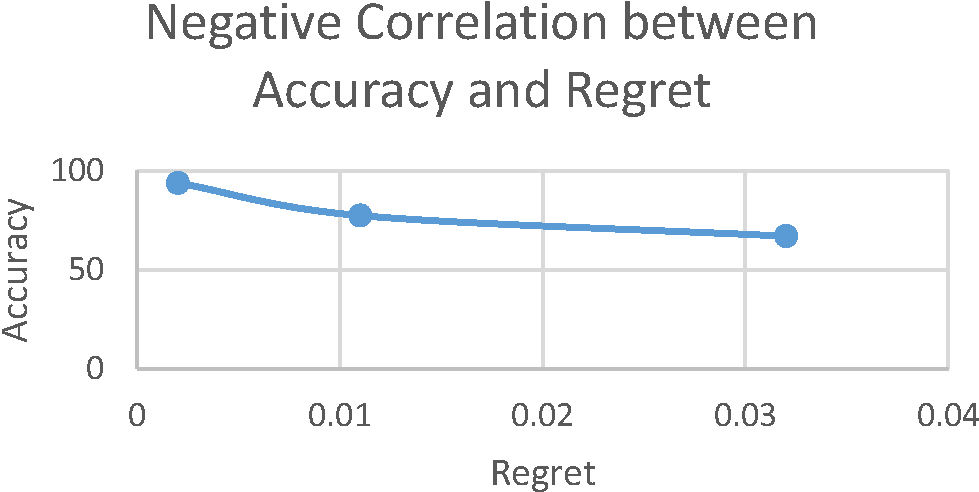
\includegraphics[width=55mm]{res/negCorrelationRegret-cropped.pdf}
			\end{center}
			
		\end{subfigure} &
		\begin{subfigure}{0.5\textwidth}
			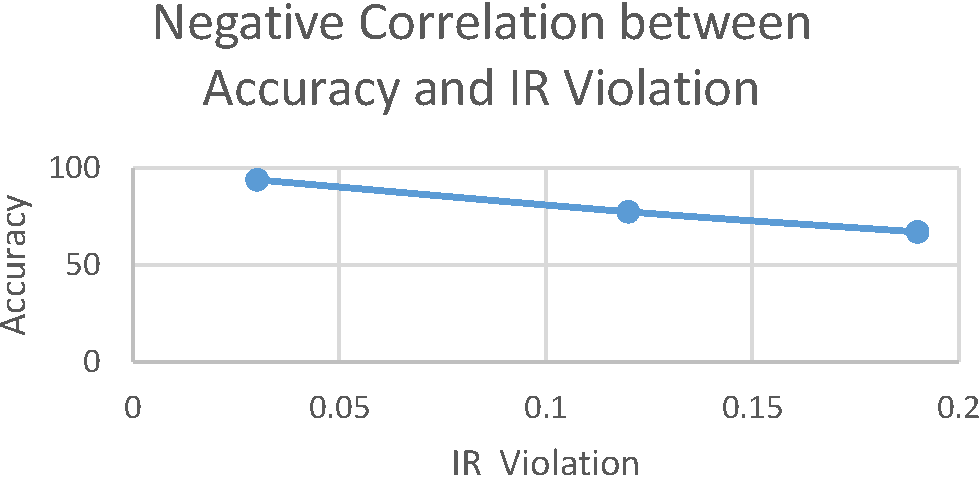
\includegraphics[width=55mm]{res/negCorrelationIR-cropped.pdf}
		\end{subfigure}
	\end{tabular}
	\caption{Correlation between accuracy and regret / ir violation}
	\label{accuracyCorrelation}
\end{figure}
\vspace{-5mm}
\paragraph{Degree of complementarity} has a major effect on the results. Regret is higher for low complementarity between the items and it generally leads to less predictable allocations (Fig. \ref{degComplementarity}).
\begin{figure}[!ht]
		\begin{tabular}{c c c}
		\begin{subfigure}{0.3\textwidth}
			
			\begin{center}
				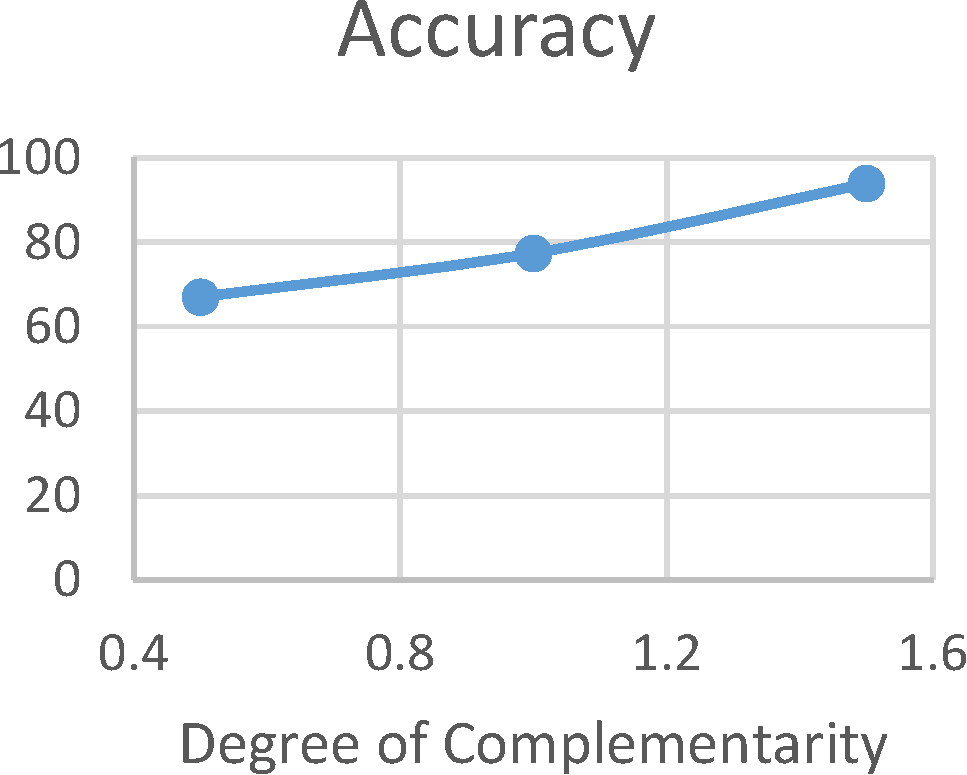
\includegraphics[width=38mm]{res/degComplementarity_accuracy-cropped.pdf}
			\end{center}
			
		\end{subfigure} &
	\begin{subfigure}{0.3\textwidth}
		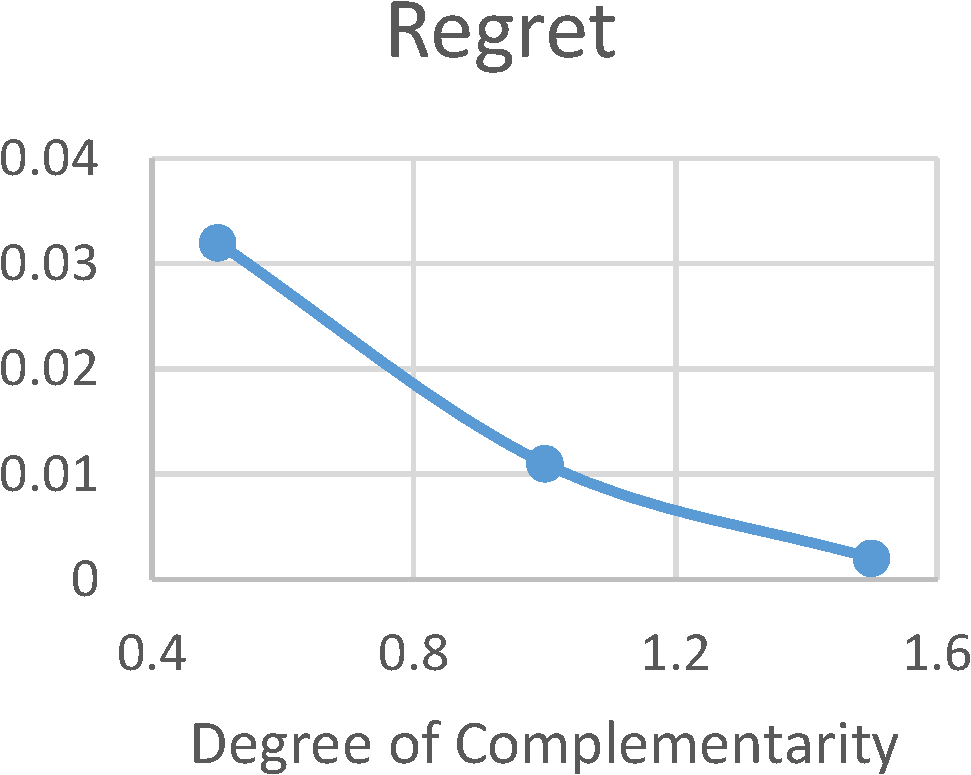
\includegraphics[width=38mm]{res/degComplementarity_regret-cropped.pdf}
	\end{subfigure} &
\begin{subfigure}{0.3\textwidth}
	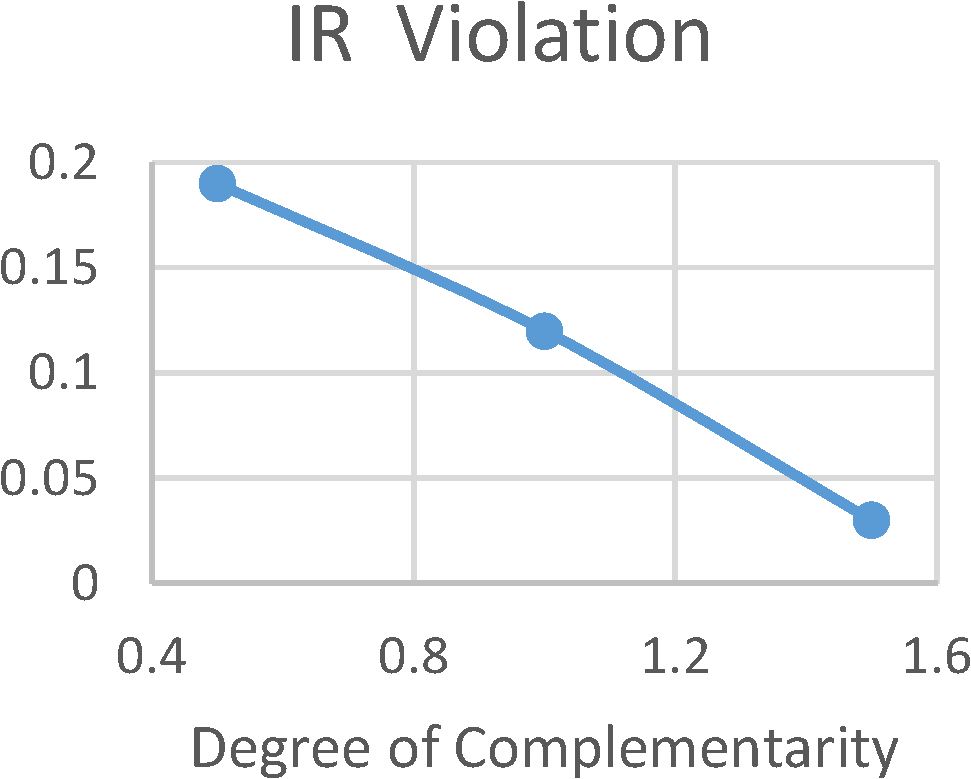
\includegraphics[width=38mm]{res/degComplementarity_ir-violation-cropped.pdf}
\end{subfigure}
\end{tabular}
\caption{Effect of degree of complementarity on accuracy, regret and ir violation}
\label{degComplementarity}
\end{figure}
\vspace{-5mm}
\paragraph{Choice of the outcome rule} in combination with the choice of an attribute mapping function also leads to significant differences in the outcome (Fig. \ref{choiceOutAttr}). Attribute mapping function $\chi$ maps input and output into a single vector.
\begin{figure}[!ht]
	\begin{tabular}{c c}
		\begin{subfigure}{0.5\textwidth}
			\begin{center}
				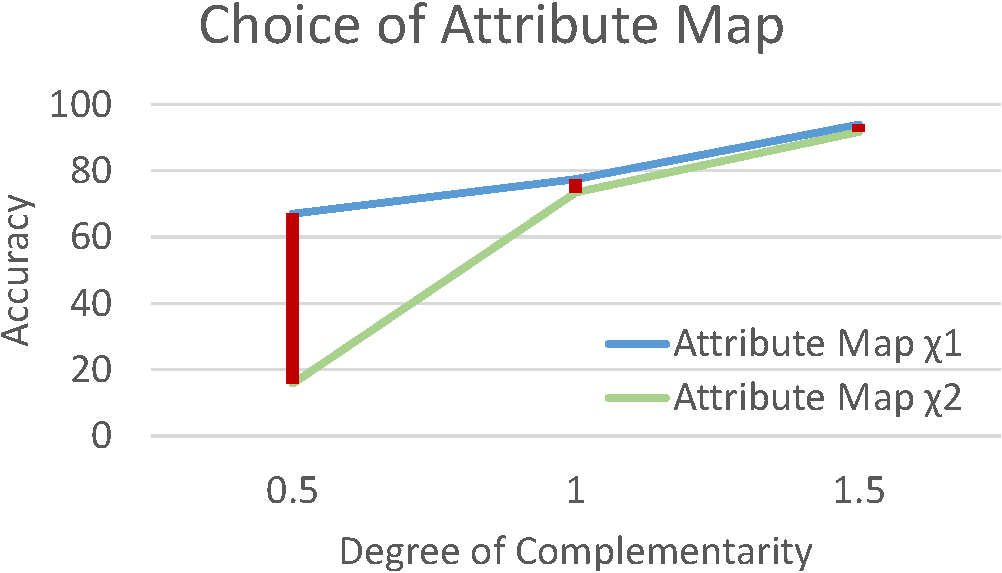
\includegraphics[width=55mm]{res/choiceAttributeMap-cropped.pdf}
			\end{center}
		\end{subfigure} &
		\begin{subfigure}{0.5\textwidth}
			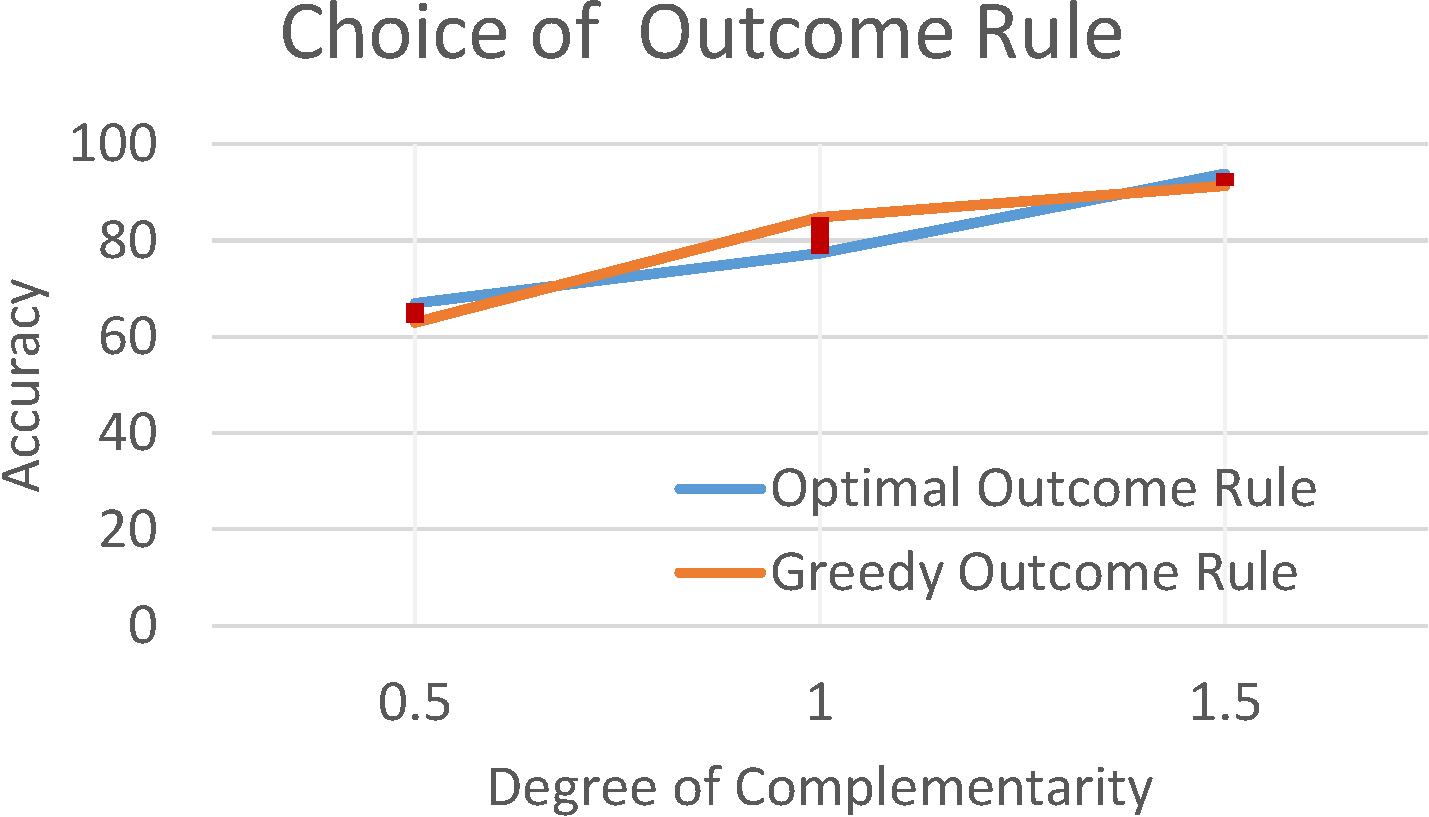
\includegraphics[width=55mm]{res/choiceOutcomeRule-cropped.pdf}
		\end{subfigure}
	\end{tabular}
	\caption{Effect of choosing a different outcome rule or attribute map}
	\label{choiceOutAttr}
\end{figure}

\paragraph{Increase the size of the training set}  leads to overall better results. In the experiments training sets with the sizes 100, 300 and 500 were used.

\paragraph{IR Fixes} payment offset, adjusting loss function and introducing deallocation decrease \emph{ir-violation} but unfortunately regret tends to move in the opposite direction.

\section{Conclusion}
In the introduction we were looking at three challenges that the classical approach brings: computational complexity, exclusion of mechanisms and analytical complexity. Now we are going to reflect back on if and how the new approach overcomes them.

\paragraph{Analytical Complexity} It is hard to tell in general if this complexity is really reduced with the new approach.
Because it is still not a framework that a mechanism designer can plug into any situation without additional effort. As an example, the mechanism designer has to find a good attribute mapping function and as we've seen this choice has a significant effect on the outcome.

\paragraph{Exclusion of Mechanisms} Mechanisms with useful economic properties that were precluded because of the hard IC constraint are possible now with the new approach because a hard IC constraint doesn't exist any more.

\paragraph{Computational Complexity} The computational cost associated with the new approach occurs offline during training. The learned payment rules have a succinct description and can be evaluated quickly in a deployed mechanism. \\


\noindent To summarize the paper, the authors have introduced a new paradigm for computational mechanism design, in which statistical machine learning is adopted to design payment rules for given outcome rules, and have shown encouraging experimental results. However, there are still quite a few directions of interest that have to be investigated in the future. 


\end{document}
